% Chapter 3

\chapter{Methodology} % Main chapter title

\label{Chapter3} % For referencing the chapter elsewhere, use \ref{Chapter1} 

%----------------------------------------------------------------------------------------

\section{Methods and techniques selected}
In the following sections the term “technique” is used for any procedure that can be boiled down to an algorithm, while the term “method” is used for a coherent combination of techniques.

As illustrated in figure 1.1, and further elaborated in the working definition of “software evolution” in paragraph 1.3, the methods and techniques chosen are applied to a population of software releases. Therefore, the basic entity under scrutiny, the “operational taxonomic unit” \citep{Sokal1986a}, is the “software release”.

\subsection{Data acquisition and encoding techniques}

The choice of techniques for data acquisition is based, with alterations, on the overview of software metrics provided by \citet{Nagappan2008a} reviewed in paragraph 2.2.1. \citet{Nagappan2008a} distinguish between code structure characteristics and organizational characteristics. The following characteristics were used to describe software releases.

\subsubsection{Code structure characteristics}
For the present research, it was assumed that for the study of software evolution, the most relevant code structure characteristic is a measure of code churn, redefined as the amount of change introduced by each release.

\noindent
Code churn was recorded by 2 measurements: 
\begin{itemize}
\item{The presence (or absence) of each file in each specific release.}
\item{a checksum of each file indicating file changes across releases.}
\end{itemize}

\subsubsection{Organizational characteristics}
Software source code is generally developed and stored in a code repository. Code repositories record who edited each file and who committed the change in the repository, thus providing information about the structure of the development team involved in each software release. Team structure characteristics were recorded in three measurements:

\begin{itemize}
\item{\textit{Team composition} was recorded as the presence (or absence) of a team member for each specific release.}
  
\item{\textit{Edit frequency} was recorded as the number of edits by each team member for each release. Editors contribute their knowledge to the code base, so the number of edits indicates how much knowledge is provided by a team.}

\item{\textit{Code ownership} was recorded as the number of commits by each team member for each release. Committers control which edits make it into the code base, so the number of commits indicates how much a release is owned by a team.}
\end{itemize}

\begin{table}[H]
\caption{Summary of characteristics and their data types}
\label{table:characteristics} 
\centering
\begin{tabu} to \linewidth{p{5cm} p{5cm} p{5cm}}
  \toprule
  Characteristic & Domain & Data type \\
  \midrule
  Presence (or absence) of a file in a release &
  One measurement for each version of a file in a release &
  Boolean \\
  \midrule
  File changes (checksums) &
  One measurement for each version of a file in a release &
  categorical \\
  \midrule
  Team composition &
  One measurement for each team member contributing to a release &
  Boolean \\
  \midrule
  Edit frequency &
  One measurement for each team member contributing to a release &
  integer \\
  \midrule
  Code ownership &
  One measurement for each team member contributing to a release &
  integer \\
\bottomrule
\end{tabu}
\end{table}

\subsection{Techniques for computing the distance matrix}
As discussed in the review of literature on evolutionary techniques (2.2.3), “distance matrix methods”, i.e. evolutionary techniques that use a matrix of pairwise dissimilarity between entities to estimate a classification \citep{FelsensteinJ.andFelenstein2004a} offer an approach that produces accurate results and performs well on large data sets.

The distance matrix is computed on the base of the measurements obtained using the techniques described in paragraph 3.1.1. The result is a matrix with one column and one row for each software release, were each cell contains a measure of the pairwise dissimilarity between the corresponding two releases. As the measurements used are of different data types (table \ref{table:characteristics}), a technique that can calculate the distance matrix by combining measurements of mixed data types is required. The Gower distance provided by the R-package “StatMatch” provides such an algorithm \citep{DOrazio2016}.

\subsection{Estimating the phylogeny of releases}
Having computed a distance matrix using the techniques described in paragraph 3.1.2, the next step is to estimate a phylogenetic tree that represents the relationships between the software releases studied. The choice of techniques for estimating trees is based on the reference provided by \citet{Paradis2011}, as discussed in 2.2.2. Commonly used techniques for estimating trees include:

\begin{description}
\dt{Average linkage (UPGMA)} \dd{UPGMA is a method that generates a tree based on the degree of similarity between entities \citep{Sneath1962a}, but does not imply a descent from a common ancestor. Therefore it is a “phenetic” method, i.e. the result is a hierarchical clustering of the entities under scrutiny, based on their characteristics \citep{Rohlf2013a}.}
\dt{Neighbour-Joining (NJ)} \dd{NJ is a “cladistic” method, i.e. it assumes a descent from common ancestry and seeks the tree with the fewest possible evolutionary changes, i.e. the tree with the “maximum parsimony” \citep{Rohlf2013a}. As working on trees is a complex problem, a heuristic is used to make the search more efficient: NJ seeks the tree with the shortest total branch length, i.e. the tree with the least amount of changes, and accomplishes this by iteratively re-computing the dissimilarity matrix \citep{Saitou1987a}.}
\dt{Minimum Evolution (ME)} \dd{ME is similar to NJ in its aims, but it seeks the shortest tree by applying a different heuristic: seeking the tree with the shortest overall branch length by rearranging the topology of the tree \citep{Desper2005a}.}
\end{description}

\subsection{Cophenetic distance matrix}
The cophenetic distance is the distance at which two tips of a tree combine into a single branch \citep[p.1275]{RDevelopmentCoreTeam2008a}. A cophenetic distance matrix can be calculated for the pairwise distances as represented in the tree. Cophenetic distance matrices were used here for two purposes:

\begin{description}
\dt{As a measure of accuracy} \dd{The correlation between the distance matrix (obtained from measurements) and the cophenetic distance matrix (obtained from the tree) is a way of telling how well the tree represents the data and can be used to assess the accuracy of the phylogenetic methods \citep{Sokal1986a}.}

\dt{As input for further analysis} \dd{As the cophenetic distance matrix represents the tree, it can be used as input for statistical analysis. Cophenetic matrices were used to answer the research questions, as detailed in the following paragraph.}
\end{description}

% ----------------------------------------------------------------------------------------

\section{Justification}
The practical problem (2.1) was tackled through two research questions. These research questions were answered by reformulating them as statistical hypotheses based on the trees obtained by applying the methods and techniques selected. Cophenetic distance matrices (3.1.4) were instrumental in defining these statistical hypotheses, as cophenetic distance matrices represent the trees in a way that can be used as input for statistical analysis.

\subsection{RQ1}
Research Question 1 sought to determine a threshold beyond which two diverging branches will be more likely to fork than to merge. This result was expected to provide guidance as to the preferred strategy to follow when part of the team is getting off on its own by answering the question: is a merge still practicable or is a fork unavoidable?

\definition{Null hypothesis}{The null hypothesis is that branches and forks are indistinguishable by measuring the pairwise distance between releases.}

\definition{Alternative hypothesis}{The alternative hypothesis is that a branch can be told from a fork by measuring the pairwise distance between releases.}

\noindent
These hypotheses can be translated into statistical hypotheses by examining the cophenetic distance matrix obtained from the estimated phylogenetic tree.

\definition{Statistical null hypothesis}{The statistical null hypothesis is that the mean cophenetic distances between releases on the same branch and on different forks are not significantly different.}

\definition{Alternative statistical hypothesis}{The alternative statistical hypothesis is that the mean cophenetic distance between a pair of releases is significantly different (p < 0.05) depending on whether the releases are on different forks or on the same branch.}

\subsection{RQ2}
Research Question 2 sought to determine whether the outcome of a fork can be predicted through phylogenetic methods. The predicted outcome was expected to fall into one of three categories: cooperation, competition or discontinuation. This result would provide guidance as to which outcome is to be expected in the future of the fork and which strategy is more suitable to attain the project's goals. 

The expected outcome was that two distinct but cooperating teams would produce a code base with many similarities, while two competing teams would produce clearly distinct code bases. The proposed method for answering this question is to use the same approach as in RQ1, but applying it to the two data sets obtained from code measurements and team measurements, thus estimating a “code-base tree” and a “team tree” for each fork. 

\definition{Null hypothesis}{The null hypothesis is that forks with different outcomes are indistinguishable based on code and organizational measurements.}

\definition{Alternative hypothesis}{The alternative hypothesis is that the outcome of a fork can be predicted by measuring the pairwise distances between releases, based on separate code and organizational data sets.}

\noindent
These hypotheses can be translated into statistical hypotheses by calculating the variance of the cophenetic distances between trees of forks obtained from code measurements and trees constructed from team measurements.

\definition{Statistical null hypothesis}{The statistical null hypothesis is that the mean distance between forks with different outcomes are not significantly heterogeneous with regard to the outcome of the fork.}

\definition{Alternative statistical hypothesis}{The alternative statistical hypothesis is that the mean distance between forks with different outcomes are significantly heterogeneous with regard to the outcome of the fork.}

%----------------------------------------------------------------------------------------
\section{Research procedures}
The research questions are examined by applying the activities detailed in figure \ref{fig:methods}.

\begin{figure}[H]
  \centering
  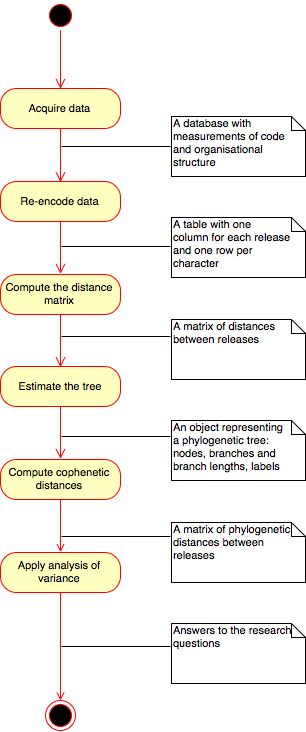
\includegraphics[width=0.5\textwidth]{methods.png}
  \caption{Activity diagram of the steps necessary for estimating phylogenetic relationships using distance-based methods, as implemented for the present research.}
  \label{fig:methods}
\end{figure}

\subsection{Data acquisition and re-encoding}
Data was acquired from selected open source repositories. The choice of software projects to study was guided by the comprehensive review of forks provided by \citet{Robles2012a}. Forks are per definition only possible in an open source context, therefore any conclusions apply in this context only. Additionally, the choice of projects was limited by the availability of a complete release history of the project, at least as far back as the moment in time were the fork happened.

As forking is a process at the crossroads between technical evolution and organizational evolution (as per the definition in paragraph 1.3), the data acquisition techniques were chosen to cover technical and organizational aspects of projects.

Data has to be re-encoded in order to be processable. This process is explained in detail in paragraph 4.1.2. Guidelines for re-encoding characters can be found in \citet{Sokal1986a}.

\subsection{Distance matrices}
As explained in paragraph 3.1.2, the chosen methods for answering the research questions are all part of the “distance matrix” family of phylogenetic methods. As shown in figure 3.1, a matrix of the pairwise dissimilarity between the releases of the chosen fork has to be computed. Several techniques are available to compute a distance matrix: computing Euclidean, or “Manhattan” distances are commonly used \citep{Felsenstein1982a}. However, these techniques are limited to processing numerical and Boolean data respectively. As the acquired data is of various data types (Boolean, categorical, numerical, see table \ref{table:characteristics}) the chosen method is required to process different data types. Only the “Gower” technique \citep{DOrazio2016} satisfies this requirement. However, the Gower technique is limited in that matrix rows with missing values do not contribute to the result, therefore, part of the data acquired was discarded before processing.

Table 3.2 shows an example distance matrix, constructed by subsampling the data collected for the Mysql / MariaDB fork (see 4.1 for details). Ten branches and thousand measurement characters were selected at random (the original data set has 107 branches and 56 648 measurement characters).

\subsection{Phylogenetic trees and cophenetic distances}
The proposed methods for answering the research questions involve constructing phylogenetic trees by applying the methods described in 3.1.3.

Figure \ref{fig:sample_tree} shows an example tree constructed using the subsample of the data presented in table 3.2. The Neighbour-Joining algorithm \citep{Saitou1987a} was used to estimate the tree.

\begin{figure}[H]
  \centering
  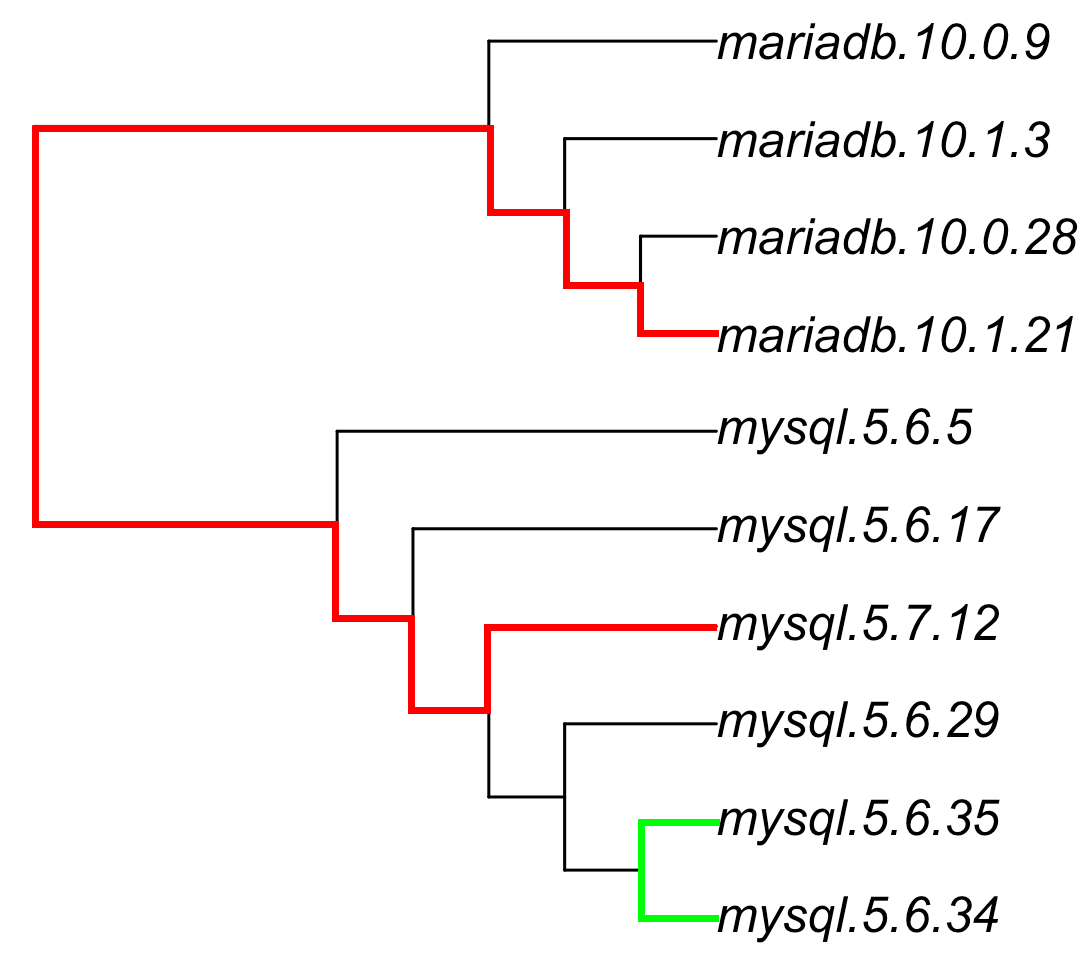
\includegraphics[width=0.5\textwidth]{mysql_sample_tree.png}
  \caption{An example tree obtained by applying the NJ method to the data in table 3, showing the longest (red) and shortest (green) distances between tips of the tree.}
  \label{fig:sample_tree}
\end{figure}

The next step is to calculate the cophenetic distances between the tips of the trees. Figure 3.2 illustrates this: the green line represents the shortest path between two tips in the example; the red line represents the longest path between two tips.

Table 3.3 shows an example cophenetic matrix. Please note that the cophenetic matrix is calculated from the tree, so the method used to estimate the tree has an effect on the cophenetic matrix. Conversely, the correlation between the distance matrix and the cophenetic matrix can be used as a measure of how accurately the tree represents the distance matrix.

The distance matrix can be shaded to show the degree of dissimilarity between releases, and the matrix can then be rearranged into clusters of the same shade. This representation was introduced by \citet{Sneath1962a} and used to discover species and genus in the data. Table 3.4 shows that in the example data, MySQL releases are close to each other, while MySQL 5.7.12 and all releases of MariaDB are the most distant from each other (light-shaded cells in the bottom row).

\subsection{Analysis of variance}
As detailed in 3.2.1, answering RQ1 requires computing a matrix of the cophenetic distances between releases and estimating if these distances correlate to forks and branches. Figure \ref{fig:example_boxplot} shows a box plot of the cophenetic distances in the example data. The plot shows that distances between tips inside either project (“Branches”) are statistically smaller than the distances between tips on different forks (“Forks”).

\begin{figure}[H]
  \centering
  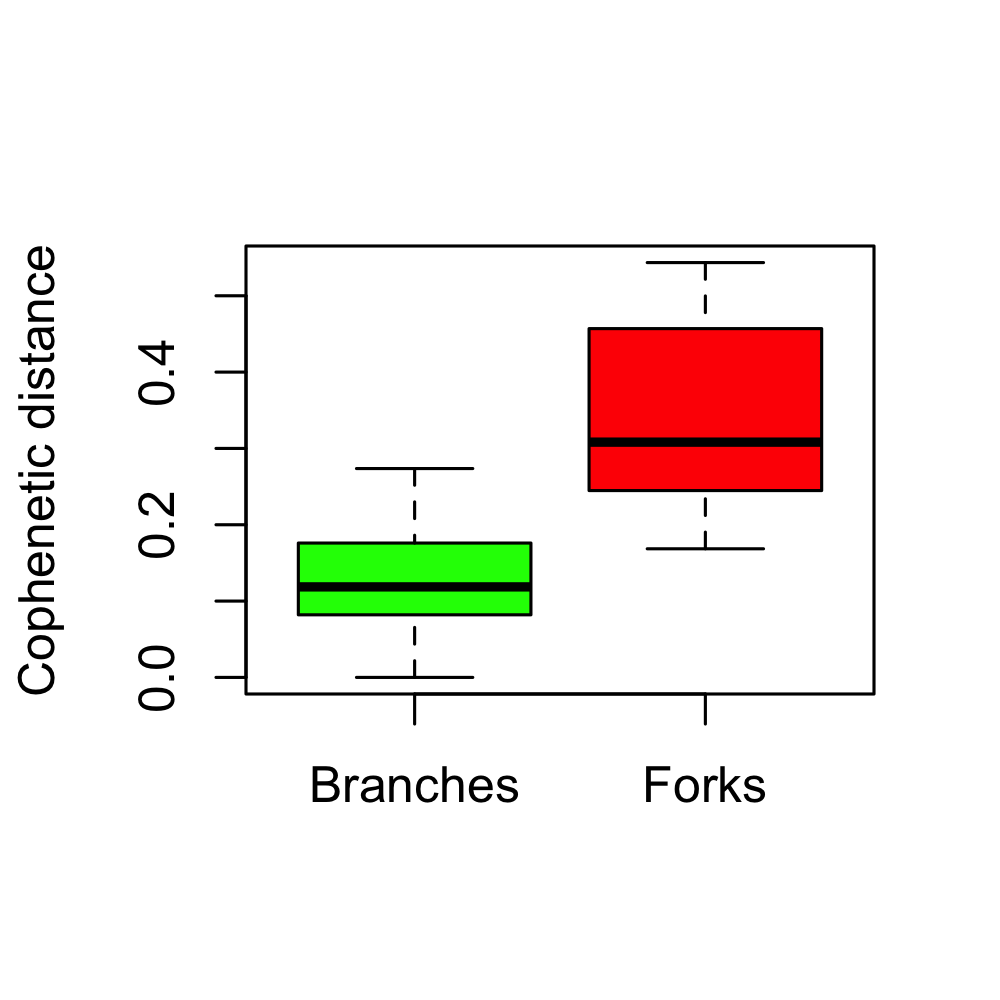
\includegraphics[width=0.5\textwidth]{example_boxplot.png}
  \caption{A box plot of the cophenetic distances of branches and forks in the example data.}
  \label{fig:example_boxplot}
\end{figure}

According to \citet{McDonald2014b}, choosing a method for statistical analysis is primarily guided by the kind and number of variables required to test the hypothesis. The cophenetic distance is a measurement variable, and whether the pairwise distance between releases corresponds to a “fork” or “branch” is a nominal variable. \citet{McDonald2014b} lists two methods for testing a hypothesis based on one measurement and one nominal variable: “student's t-test” and “analysis of variance” (ANOVA).

The method proposed for answering RQ2 (paragraph 3.2.2) requires examining projects with different outcomes and computing two cophenetic distance matrices for each project: one for the tree obtained from team measurements, and a second one for the tree obtained from code measurements. Having computed these matrices, the next step is to estimate if these distances correlate with different project outcomes. The cophenetic distance is a measurement variable, the data set used (“team measurements” or “code measurements”) is a nominal variable and the outcome of the project (“cooperation”, “competition” or “discontinuation of a branch”) is a second nominal variable. \citet{McDonald2014b} recommends applying a two-way ANOVA for testing a hypothesis based on one measurement and two nominal variables.

Consequently, RQ1 and RQ2 can be answered by applying analysis of variance (ANOVA), albeit with different number of nominal variables. ANOVA assumes that the data is normally distributed (fits the Gaussian “bell curve”) and that that the standard deviation is the same for the data sets examined, otherwise false positives may result \citep[p.147]{McDonald2014b}. As the raw data obtained from the repositories did not meet these assumptions, the data had to be transformed to fit the assumptions prior to the analysis.

%----------------------------------------------------------------------------------------
\section{Ethical considerations}
All data analysed for this research is freely available under an open source license, therefore no intellectual property rights were disregarded during the acquisition of the data. 

Some of the forks studied were a consequence of disagreements between development teams. Care was applied during the analysis not to take sides for any particular team; however, to thwart any bias ensuing from the reputation of well-known actors in the industry, all names of developers were anonymized prior to being stored locally.

Although I do participate in open source software development, I am not involved in any of the projects examined for this research.
%----------------------------------------------------------------------------------------
\section{Summary of Chapter 3}
Character measurement techniques applicable to software code bases and to software producing organizations were selected from literature. Suitable techniques to study the evolution of software were chosen from the corpus of biological techniques for estimating phylogenetic trees. The two research questions were specified in terms of hypotheses, null hypotheses and their corresponding statistical hypotheses. The steps required by the research were worked out and each step was illustrated with an example drawn from a subset of the data. Finally, analysis techniques suitable to answer the research questions were selected, based on the type and number of independent variables required by the analysis.


